\section{Version Control System}
\begin{mdframed}
    \textbf{VCS:} a component of software configuration management, is the management of changes to documents, computer programs, large web sites, and other collections of information.
\end{mdframed}

\subsection{Caratteristiche}
\begin{itemize}
    \item Sono sistemi software
    \item Registrano modifiche avvenute ad un insieme di file
    \item Condivisione di file e modifiche
    \item Funzionalità: merging, tracciamento modifiche
\end{itemize}

\subsection{Tipologie di VCS}

\subsubsection{Local VCS}
\begin{itemize}
    \item Tool più vecchi
    \item Registrano solo storia cambiamenti
    \item Non gestiscono la condivisione
    \item Esempi: SCSS, IDE(Eclipse, IntelliJ)
\end{itemize}

\subsubsection{Centralized VCS - CVCS}
\begin{itemize}
    \item Meno vecchi e molto diffusi
    \item Gestiscono sia la condivisione, che il tracciamento della storia
    \item Ogni sviluppatore è un client che ha nel suo spazio di lavoro solo una versione del codice
    \item Facili da apprendere
    \item Esempi: CVS, Subversion(SVN), Perforce, TFS
\end{itemize}

\subsubsection{Distributed VCS - DVCS}
\begin{itemize}
    \item Version Database distribuito per duplicazione in ogni nodo
    \begin{itemize}
        \item quando il nodo principale non è disponibile, è possibile continuare a lavorare e registrare i cambiamenti
        \item migliore risoluzione dei conflitti
        \item diversi tipi di flussi di lavoro
    \end{itemize}
    \item Difficili da apprendere
    \item Esempi: Git, Mercurial
\end{itemize}

\subsubsection{Cloud-Based DVCS}
\begin{itemize}
    \item VCS as a Service
    \item Version Database gestito in un servizio Cloud
    \item Esempi: GitHub, GitLab
\end{itemize}

\subsection{Nozioni}
\begin{itemize}
    \item \textbf{DIFF:} each set of changed lines
    \item \textbf{COMMIT:} set of DIFF
    \item \textbf{HEAD:} last commit
    \item \textbf{BRANCH:} pointer to a single commit
    \begin{itemize}
        \item HEAD is the latest branch, know as \textbf{main} branch
        \item to integrate a branch, you have to merge it
    \end{itemize}
    \item \textbf{PULL REQUEST:} way of handling branch merges to main
    \begin{enumerate}
        \item branch pushed to the central server
        \item ask to be merged on a central repo
        \item review change before merging
        \item pull request closed or merged to destination branch
    \end{enumerate}
\end{itemize}

\subsection{Tipologie di Workflow}

\subsubsection{Centralized WF}
\begin{itemize}
    \item Utilizzo naturale di un CVCS come SVN o CVS
    \item Facile da capire e da usare
    \item Collaborazione bloccata quando il server centralizzato è fuori uso o la cronologia è interrotta
\end{itemize}
\begin{center}
    \begin{tabular}{c}
        \\ 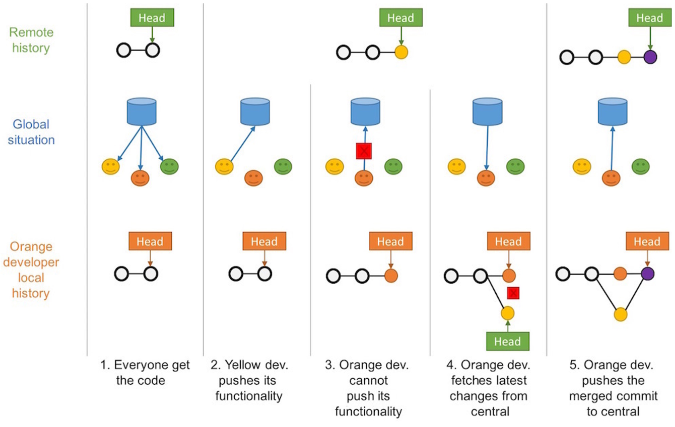
\includegraphics[width=0.9\textwidth]{images/VCS1.png} \\ \\
    \end{tabular}
\end{center}

\newpage
\subsubsection{Feature Branch WF}
\begin{itemize}
    \item L'obiettivo è quello di utilizzare un solo ramo per caratteristica (DVCS)
    \item L'incapsulamento consente di lavorare senza distribuire la base di codice principale
    \item Collaborazione più facile
    \item Più facile da tracciare
\end{itemize}
\begin{center}
    \begin{tabular}{c}
        \\ 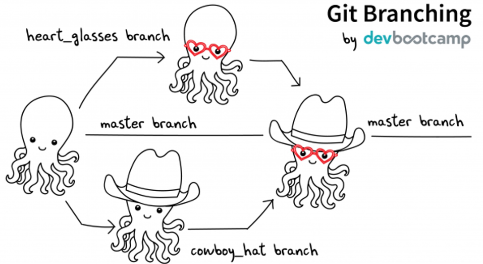
\includegraphics[width=0.7\textwidth]{images/VCS2.png} \\ \\
    \end{tabular}
\end{center}

\subsubsection{Gitflow Model WF}
\begin{itemize}
    \item main branch: codice rilasciato
    \item developer branch: snapshot per la prossima release
    \item feature branch: nuova funzionalità
\end{itemize}
\begin{center}
    \begin{tabular}{c}
        \\ 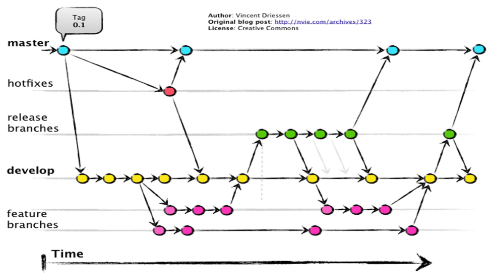
\includegraphics[width=0.9\textwidth]{images/VCS3.png} \\ \\
    \end{tabular}
\end{center}

\subsubsection{GitHub Flow}
\begin{itemize}
    \item Approccio più veloce di sviluppo
    \item Focalizzato sulle caratteristiche per unire i nuovi rami con il ramo master
    \item Flusso di lavoro perfetto per piccoli team e progetti
\end{itemize}
\begin{center}
    \begin{tabular}{c}
        \\ 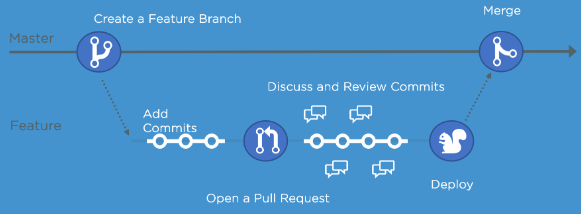
\includegraphics[width=0.9\textwidth]{images/VCS4.png} \\ \\
    \end{tabular}
\end{center}

\subsubsection{GitLab Flow}
\begin{itemize}
    \item Approccio di sviluppo più attento all'affidabilità
    \item Processo di test a più fasi
\end{itemize}
\begin{center}
    \begin{tabular}{c}
        \\ 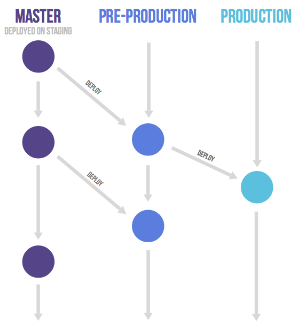
\includegraphics[width=0.5\textwidth]{images/VCS5.png} \\ \\
    \end{tabular}
\end{center}

\newpage
\subsubsection{Forking WF}
\begin{itemize}
    \item Concetti di push forward del file system distribuito
    \item Ogni utente fa il fork del repo principale e può proporre richieste di pull tra i repo
    \item Gestione delle autorizzazioni migliorata
    \item Autonomia per un migliore processo di collaborazione
    \item Decentrato per nuovi modelli
\end{itemize}
\begin{center}
    \begin{tabular}{c}
        \\ 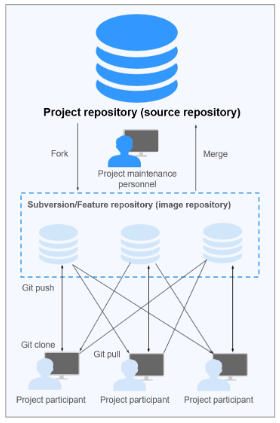
\includegraphics[width=0.5\textwidth]{images/VCS6.png} \\ \\
    \end{tabular}
\end{center}

\subsection{CVCS vs DVCS}
\begin{multicols}{2}
    \raggedright
    \textbf{CVCS:}
    \begin{itemize}
        \item[+] apprendimento più semplice
        \item[+] lock file
        \item[-] meno recenti
        \item[-] centralized workflow
        \item[-] commit più lenti
        \item[-] single point of failure
    \end{itemize}
    \columnbreak
    \textbf{DVCS:}
    \begin{itemize}
        \item[+] più recenti
        \item[+] distribuiti
        \item[+] migliori workflow
        \item[+] commit veloci
        \item[-] no lock file
        \item[-] apprendimento difficile
    \end{itemize}
\end{multicols}

\newpage